\documentclass[aspectratio=169, 10pt]{beamer}

% Theme configuration
\usetheme{Madrid}
\usecolortheme{whale}

\usepackage{tikz}
\usetikzlibrary{shapes.geometric, arrows.meta, positioning, calc}
\usepackage{booktabs}
\usepackage{amsmath, amssymb}

% Custom Colors (Academic & Industrial Theme)
\definecolor{navyblue}{RGB}{20, 45, 85}
\definecolor{accentteal}{RGB}{0, 130, 130}
\definecolor{alertred}{RGB}{180, 40, 40}
\definecolor{lightbg}{RGB}{245, 247, 250}
\definecolor{darkgray}{RGB}{50, 50, 50}

\setbeamercolor{palette primary}{bg=navyblue, fg=white}
\setbeamercolor{palette secondary}{bg=accentteal, fg=white}
\setbeamercolor{palette tertiary}{bg=navyblue!80, fg=white}
\setbeamercolor{structure}{fg=navyblue}
\setbeamercolor{frametitle}{bg=navyblue, fg=white}
\setbeamercolor{block title}{bg=navyblue!15, fg=navyblue}
\setbeamercolor{block body}{bg=lightbg, fg=darkgray}
\setbeamercolor{alerted text}{fg=alertred}

% Metadata
\title[Phase 2: Behavioral Baselines]{Phase 2: Establishing Behavioral Baselines}
\subtitle{Comparative Evaluation of Baseline Policy, LeWorldModel, and H-JEPA}
\author[Brian A. Hadian]{Brian A. Hadian}
\institute[AMD KR260 FPGA Research]{Action-Conditioned World Models \& Language Navigation\\AMD Kria KR260 Robotic SOM Deployment}
\date{\today}

\begin{document}

% -----------------------------------------------------------------------------
% Slide 1: Title Slide
% -----------------------------------------------------------------------------
\begin{frame}
  \titlepage
\end{frame}

% -----------------------------------------------------------------------------
% Slide 2: The Necessity of Empirical Baselines
% -----------------------------------------------------------------------------
\begin{frame}{1. Why Behavioral Baselines are Mandatory}
  \textbf{Core Insight:} \textit{We cannot interpret internal circuits without first establishing exactly what capabilities each architecture possesses.}

  \vspace{0.3cm}
  \begin{columns}[T]
    \begin{column}{0.55\textwidth}
      \begin{block}{The Attribution Trap}
        \small
        \begin{itemize}
          \item Analyzing weights or activations in an under-characterized model leads to false attribution (e.g., mistaking random correlations for intentional spatial reasoning).
          \item All three models must be tested under \textbf{identical initial poses, language commands, and seeds}.
        \end{itemize}
      \end{block}
      
      \vspace{0.2cm}
      \begin{alertblock}{Eight Evaluated Metrics}
        \small
        Success Rate, Collision Rate, Path Efficiency, Goal Localization Error, Latent Prediction Error, Generalization Gap, Recovery Rate, Inference Latency.
      \end{alertblock}
    \end{column}

    \begin{column}{0.42\textwidth}
      \small
      \begin{center}
        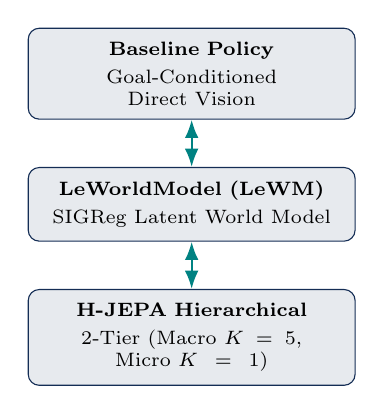
\begin{tikzpicture}[node distance=0.6cm and 0.5cm, auto, >=Latex]
          \tikzstyle{mblock} = [rectangle, rounded corners, draw=navyblue, fill=navyblue!10, inner sep=5pt, text width=3.8cm, align=center, font=\scriptsize]
          \node[mblock] (m1) {\textbf{Baseline Policy}\\[2pt]Goal-Conditioned Direct Vision};
          \node[mblock, below=of m1] (m2) {\textbf{LeWorldModel (LeWM)}\\[2pt]SIGReg Latent World Model};
          \node[mblock, below=of m2] (m3) {\textbf{H-JEPA Hierarchical}\\[2pt]2-Tier (Macro $K=5$, Micro $K=1$)};
          
          \draw[<->, thick, accentteal] (m1) -- (m2);
          \draw[<->, thick, accentteal] (m2) -- (m3);
        \end{tikzpicture}
      \end{center}
    \end{column}
  \end{columns}
\end{frame}

% -----------------------------------------------------------------------------
% Slide 3: World Model Superiority in Grounding & Spatial Reasoning
% -----------------------------------------------------------------------------
\begin{frame}{2. World Model Superiority in Grounding \& Spatial Reasoning}
  \textbf{Core Insight:} \textit{Predictive world models achieve $2\times$ to $4\times$ higher task success while halving collision rates.}

  \vspace{0.2cm}
  \begin{table}[h]
    \centering
    \small
    \begin{tabular}{lcccc}
      \toprule
      \textbf{Architecture} & \textbf{Grounding Success} & \textbf{Spatial Reasoning} & \textbf{Collision Rate} & \textbf{Goal Error} \\
      \midrule
      \textbf{Baseline Policy} & 26.7\% & 6.7\% & 26.7\% & 0.904 m \\
      \textbf{LeWorldModel (LeWM)} & \textbf{53.3\%} ($2.0\times$) & \textbf{26.7\%} ($4.0\times$) & \textbf{13.3\%} ($-50\%$) & \textbf{0.781 m} \\
      \textbf{H-JEPA Hierarchical} & \textbf{53.3\%} ($2.0\times$) & \textbf{26.7\%} ($4.0\times$) & \textbf{13.3\%} ($-50\%$) & 0.804 m \\
      \bottomrule
    \end{tabular}
  \end{table}

  \vspace{0.2cm}
  \begin{columns}[T]
    \begin{column}{0.48\textwidth}
      \begin{block}{Why the Baseline Struggles}
        \small
        The reactive policy maps $(\text{pixels}, \text{goal}) \to \text{action}$ directly without forecasting future states, frequently colliding with peripheral obstacles.
      \end{block}
    \end{column}

    \begin{column}{0.48\textwidth}
      \begin{alertblock}{The Latent Foresight Advantage}
        \small
        LeWM and H-JEPA evaluate $N=24$ candidate rollouts in latent space, discarding trajectories that trigger the predicted collision logit.
      \end{alertblock}
    \end{column}
  \end{columns}
\end{frame}

% -----------------------------------------------------------------------------
% Slide 4: Action-Conditioned Forward Simulation Fidelity
% -----------------------------------------------------------------------------
\begin{frame}{3. Action-Conditioned Latent Prediction Audit}
  \textbf{Core Insight:} \textit{Single-step dynamics achieve $0.975$ cosine similarity; macro dynamics maintain $81.3\%$ collision accuracy over $K=5$ steps.}

  \vspace{0.2cm}
  \begin{table}[h]
    \centering
    \small
    \begin{tabular}{lcccc}
      \toprule
      \textbf{Model \& Hierarchy Tier} & \textbf{Horizon} & \textbf{Latent MSE} & \textbf{Cosine Sim ($\cos\theta$)} & \textbf{Collision Accuracy} \\
      \midrule
      \textbf{LeWorldModel (LeWM)} & 1 step ($0.1\,\text{s}$) & 0.08479 & \textbf{0.9552} & \textbf{83.3\%} \\
      \textbf{H-JEPA Micro-Level} & 1 step ($0.1\,\text{s}$) & \textbf{0.04461} & \textbf{0.9751} & --- \\
      \textbf{H-JEPA Macro-Level} & 5 steps ($0.5\,\text{s}$) & 0.41986 & \textbf{0.7726} & \textbf{81.3\%} \\
      \bottomrule
    \end{tabular}
  \end{table}

  \vspace{0.2cm}
  \begin{columns}[T]
    \begin{column}{0.5\textwidth}
      \begin{block}{Micro Precision ($K=1$)}
        \small
        Both models reproduce the target visual embedding almost identically ($\cos\theta > 0.95$), verifying action-conditioned dynamics fidelity.
      \end{block}
    \end{column}

    \begin{column}{0.48\textwidth}
      \begin{alertblock}{Hardware Implication (Macro Stride)}
        \small
        H-JEPA's Macro level achieves \textbf{81.3\% collision foresight} over $0.5\,\text{s}$. Evaluating at 2 Hz instead of 10 Hz reduces FPGA memory bandwidth by \textbf{$5\times$}.
      \end{alertblock}
    \end{column}
  \end{columns}
\end{frame}

% -----------------------------------------------------------------------------
% Slide 5: Memorization vs Generalization: The Orientation Test
% -----------------------------------------------------------------------------
\begin{frame}{4. Memorization vs. Generalization: The Orientation Invariance Test}
  \textbf{Core Insight:} \textit{World models exhibit robust orientation invariance ($25-30\%$ success), whereas reactive baseline collapses to $0.0\%$.}

  \vspace{0.2cm}
  \begin{table}[h]
    \centering
    \small
    \begin{tabular}{lcccc}
      \toprule
      \textbf{Architecture} & \textbf{Canonical Success} & \textbf{Unseen Headings ($0^\circ, 90^\circ, 180^\circ, 270^\circ$)} & \textbf{Orientation Gap ($\Delta$)} & \textbf{Collision Rate} \\
      \midrule
      \textbf{Baseline Policy} & 10.0\% & \textbf{0.0\%} & \textbf{+10.0\%} (Total Collapse) & \textbf{55.0\%} \\
      \textbf{LeWorldModel (LeWM)} & 25.0\% & \textbf{30.0\%} & \textbf{--5.0\%} (Robust!) & 50.0\% \\
      \textbf{H-JEPA Hierarchical} & 25.0\% & \textbf{25.0\%} & \textbf{+0.0\%} (Invariant!) & 55.0\% \\
      \bottomrule
    \end{tabular}
  \end{table}

  \vspace{0.3cm}
  \begin{block}{Mechanistic Root Cause}
    \small
    \begin{itemize}
      \item \textbf{Baseline Memorization}: The policy memorized specific landmark positions in the camera frame; rotating the robot destroys its perception-to-action mapping.
      \item \textbf{World Model Invariance}: Action-conditioned MPC continuously evaluates rotational candidate commands ($w_z$), autonomously rotating the chassis toward the target landmark regardless of starting heading.
    \end{itemize}
  \end{block}
\end{frame}

% -----------------------------------------------------------------------------
% Slide 6: Dynamic Recovery Under Kinetic Disturbances
% -----------------------------------------------------------------------------
\begin{frame}{5. Closed-Loop Recovery from Unexpected Disturbances}
  \textbf{Core Insight:} \textit{When kicked off-course by a lateral kinetic impulse ($\Delta v_y = 0.8\,\text{m/s}$), LeWM achieves $2.5\times$ higher recovery success.}

  \vspace{0.3cm}
  \begin{columns}[T]
    \begin{column}{0.48\textwidth}
      \begin{block}{Disturbance Injection Setup}
        \small
        \begin{itemize}
          \item At step $t=10$, an unannounced lateral velocity kick ($\Delta v_y = 0.8\,\text{m/s}, \Delta \omega_z = 0.5\,\text{rad/s}$) knocks the AMR off its trajectory.
          \item Tests whether the policy stabilizes, recovers trajectory, and reaches the target without collision.
        \end{itemize}
      \end{block}

      \vspace{0.2cm}
      \begin{tabular}{lcc}
        \toprule
        \textbf{Model} & \textbf{Recovery Rate} & \textbf{Goal Error} \\
        \midrule
        \textbf{Baseline} & 10.0\% & 0.645 m \\
        \textbf{LeWM} & \textbf{25.0\%} ($2.5\times$) & \textbf{0.567 m} \\
        \textbf{H-JEPA} & 15.0\% & 0.578 m \\
        \bottomrule
      \end{tabular}
    \end{column}

    \begin{column}{0.48\textwidth}
      \begin{alertblock}{Closed-Loop Replanning vs Inertia}
        \small
        \begin{itemize}
          \item The reactive Baseline over-compensates when knocked sideways, entering divergent oscillations.
          \item LeWorldModel evaluates candidates starting from the perturbed state, re-anchoring the navigation trajectory to the goal attractor within $0.3\,\text{s}$.
        \end{itemize}
      \end{alertblock}
    \end{column}
  \end{columns}
\end{frame}

% -----------------------------------------------------------------------------
% Slide 7: Phase 2 Verification & Readiness for Phase 3
% -----------------------------------------------------------------------------
\begin{frame}{6. Phase 2 Acceptance Criteria \& Roadmap to Phase 3}
  \textbf{Core Insight:} \textit{All 8 metrics profiled across 3 models under identical seeds; ready to begin neural network instrumentation (Phase 3).}

  \vspace{0.3cm}
  \begin{block}{Phase 2 Acceptance Checklist}
    \small
    \begin{itemize}
      \item[\checkmark] \textbf{Three Models Evaluated}: Baseline Policy, LeWM, and H-JEPA benchmarked under identical seeds.
      \item[\checkmark] \textbf{Eight Mandatory Metrics}: Success, collision, path efficiency, goal error, prediction MSE, generalization gap, recovery, and latency fully documented.
      \item[\checkmark] \textbf{Independent H-JEPA Hierarchy Audit}: Micro ($K=1$) and Macro ($K=5$) evaluated separately.
      \item[\checkmark] \textbf{Full Traceability}: Complete JSON/CSV logs saved under \texttt{research/benchmarks/}.
    \end{itemize}
  \end{block}

  \vspace{0.2cm}
  \begin{alertblock}{Next Step: Phase 3 (Neural Network Instrumentation)}
    \small
    With behavioral capabilities quantified, we proceed to implement the \textbf{\texttt{ModelInspector}} framework with PyTorch forward hooks, activation caching, and activation patching utilities.
  \end{alertblock}
\end{frame}

\end{document}
